%%
%% Author: Berk
%% 3/21/2019
%%

% Preamble
\documentclass[11pt]{article}

% Packages
\usepackage{amsmath}
\usepackage[margin=1in]{geometry}
\usepackage{amsmath,amsthm,amssymb}
\usepackage{comment}
\usepackage[acronyms]{glossaries}
\usepackage{graphicx}
\usepackage{tikz}
\usepackage{subcaption}
\usepackage{tikz-3dplot}
\usetikzlibrary{shapes.geometric}

\newacronym{sdp}{SDP}{semidefinite program}
\newacronym{ceg}{CEG}{Convex Engineering Group}
\newacronym{gp}{GP}{Geometric Program}
\newacronym{mc}{MC}{Monte Carlo}
\newacronym{sp}{SP}{Signomial Program}
\newacronym{rgp}{RGP}{Robust Geometric Program}
\newacronym{rsp}{RSP}{Robust Signomial Program}
\newacronym{ro}{RO}{Robust Optimization}
\newacronym{so}{SO}{Stochastic Optimization}
\newacronym{mdo}{MDO}{Multidisciplinary Design Optimization}
\newacronym{dc}{DC}{difference-of-convex}
\newacronym{nlp}{NLP}{Nonlinear Program}
\newacronym{rhs}{RHS}{right hand side}
\newacronym{lhs}{LHS}{left hand side}
\newacronym{cv}{CV}{coefficient of variation}
\newacronym{srm}{SRM}{solid rocket motor}
\newacronym{sos}{SOS}{sum of squares}

\makeglossaries

% Document
\begin{document}

    \title{SDP relaxations for solid rocket motor shape optimization}
    \author{Berk Ozturk}
    \maketitle

        \section{Introduction}

    Shape optimization is inherently an infinite-dimensional problem,
    for which tractable formulations are of particular interest.
    It appears in a range of problems in aerospace design, and most notably
    aerostructural optimization which has been the bread-and-butter of the \gls{mdo} field.

    These is very little literature, if any, on solid rocket conceptual design,
    for several reasons. (1) The physics governing internal reactive flow is extremely complex,
    and there are no open-source tools that don't require domain knowledge and
    can efficiently simulate such a scenario.
    (2) There are few entities that design and build solid rocket motors, and since they have
    large amounts of resources and time and little competition there has been no impetus
    improve solid rocket design methods. (3) Solid rocket motors are relatively limited
    in capability because their burn rate is almost completely uncontrollable other
    than by properly designing the internal geometry of the rocket or actuating the
    throat of the nozzle. For this reason liquid propellant rockets have been preferred for
    many applications. (4) Rocket design is often proprietary due to arms regulations.

    This is an interesting problem where a \gls{sdp} for geometry design,
    coupled with first-order flow models may offer a good alternative to
    more traditional gradient-based methods which are used alongside
    high-fidelity internal flow simulations.
    Furthermore, problems of the form I pose appear in other interesting
    aerospace problems, such as hypersonic vehicle external geometry design,
    so the formulation has valuable extensions.


    \section{Brief background on solid rocket motors}

A \gls{srm} is extremely simple. Think a candle with a casing on it to contain the pressure and hot gas from burning material,
and a nozzle at the end to make the high-pressure flow go supersonic and generate thrust.
There are a few differences between \gls{srm}s and candles.
First is the fact that solid rocket motor fuel contains propellant and oxidizer (wax and oxygen),
whereas a candle only contains fuel and relies on an external source of oxygen (eg. the air around it).
As a result, \gls{srm}s can even be lit underwater or in a vacuum;
they are extremely robust. The second difference is the geometry.
A candle is akin to an end-burning rocket; the wax only burns at the candle's melty end.
A \gls{srm} usually has some geometry down the bore of the rocket which runs all the way down its length for greater surface area.
(An end-burning rocket is almost completely uninteresting since there is not a significant aspect of geometry to design.)
The third is the presence of the nozzle. Without it, the flow would stay sonic when exiting the bore and
not generate thrust effectively. The disadvantage of solid rocket motors is that
they are essentially a runaway chemical reaction, an explosive that is confined in a casing,
whose rate is controlled by the area of the throat of the nozzle.
Once lit, they cannot be stopped or controlled, like liquid rockets or jet engines
can be by modulating the amount of propellant and oxidizer.
Therefore the design of the geometric pattern in a \gls{srm}'s bore is critical for a proper burn rate.


    \section{Approach}

I developed a two-stage approach to the \gls{srm} design problem.
The first stage is a 1D quasi-steady rocket optimization model,
which determines both the internal flow quantities and a basic description
of the internal geometry. The model takes the following inputs:
\begin{itemize}
    \item Coarse time and spatial discretization of the rocket sections
    \item The desired thrust profile of the rocket
    \item Bounds on the rocket external dimensions, if desired
    \item Material properties of the propellant
\end{itemize}

\tdplotsetmaincoords{50}{130}
\tdplotsetrotatedcoords{0}{90}{0}

\begin{figure}
    \begin{center}
        \begin{tikzpicture}[tdplot_main_coords]
            \draw[thick,->] (0,0,0) -- (1,0,0) node[anchor=north east]{$l$};
            \draw[thick,->] (0,0,0) -- (0,-1,0) node[anchor=south west]{$r$};
            \draw[thick,dashed] (0,0,0) -- (-4,0,0) node[anchor=north west]{$$};
            % Blue circles
            \tdplotdrawarc[tdplot_rotated_coords, color=blue]{(0,0,-4)}{2}{0}{360}{anchor=south west}{$\pi r^2$};
            \tdplotdrawarc[tdplot_rotated_coords, color=blue]{(0,0,0)}{2}{0}{360}{anchor=south west}{$$};
            % Blue dashed lines
            \draw[thick,dashed,color=blue] (0,-1.414,1.414) -- (-4,-1.414,1.414) node[anchor=south east]{$l_{\rm{sec}}$};
            \draw[thick,dashed,color=blue] (0,1.414,-1.414) -- (-4,1.414,-1.414) node[anchor=north west]{$l_{\rm{sec}}$};

            % Tophalf, top circle
            \tdplotdrawarc[tdplot_rotated_coords, color=red]{(-0.25,0.25,-4)}{1}{25}{248}{anchor=north west}{$$};
            % Top half, bottom circle
            \tdplotdrawarc[tdplot_rotated_coords, color=red]{(0.25,-0.25,-4)}{1}{205}{428}{anchor=north west, right=0.5cm, above=0.5cm}{$A_{in}$};
            % Bottom half, top circle
            \tdplotdrawarc[tdplot_rotated_coords, color=red]{(-0.25,0.25,0)}{1.25}{28}{243}{anchor=north west}{$$};
            % Bottom half, bottom circle
            \tdplotdrawarc[tdplot_rotated_coords, color=red]{(0.25,-0.25,0)}{1.25}{208}{425}{anchor=north west, right=0.5cm}{$A_{out}$};

            % Red dashed lines
            \draw[thick,dashed,color=red] (0,-0.85,0.85) -- (-4,-0.67,0.67) node[anchor=south east]{$$};
            \draw[thick,dashed,color=red] (0,0.85,-0.85) -- (-4,0.67,-0.67) node[anchor=north west]{$$};
        \end{tikzpicture}
    \end{center}
    \caption{Labeling of a single section of the rocket. }
    \label{fig:SRMsection}
\end{figure}

The optimization model, which is a signomial (i.e. difference-of-log-convex) program, determines the
flow properties inside and thrust generated by a rocket that has
been partitioned into $n_x$ of sections that evolve in $n_t$ time steps.
I don't want to bore you with the details, but this was possible by performing a
relaxation on all three conservation laws (mass, momentum and energy),
and writing the 1D finite volume approximation of the reactive flow problem
as a signomial program in GPkit\footnote{GPkit is an open-source modeling framework
that abstracts away solvers, and facilitates the use of geometric and signomial programs in engineering design.}.
Figure~\ref{fig:SRMsection} shows a potential cross-section of such a \gls{srm}.
The physical model assumes quasi-steady flow during each timestep, where the fluid travels strictly
in the $l$ direction down the bore drawn in red, and the conservation laws are enforced at
each bore cross-sectional area $A$. The output variables of this model are:
\begin{itemize}
    \item The material properties of the fuel burned in a given section in one time step, which are:
    \begin{itemize}
        \item Porosity of fuel
        \item Mass fraction of propellant
        \item Mass fraction of accelerant
        \item Mass fraction of filler
    \end{itemize}
    \item The arc lengths of shapes of $A_{in}$ and $A_{out}$
    \item The cross-sectional areas of $A_{in}$ and $A_{out}$
\end{itemize}

The idea is to take these output variables, and map them onto a series of
non-intersecting univariate polynomials $p_{i,t}(\theta), i = [1,2,...,n_x], t = [1,...,n_t]$
which describe the internal geometry of the rocket.
Another idea was to map to the bivariate polynomial $p_i(\theta,t)$
which has the requirement to be monotonically increasing in $t$
but I stuck to univariate polynomials since the problem
was difficult enough.
To give context about the kinds of cross-sectional shapes that are currently used in rocket design,
see Figure~\ref{fig:potentialShapes}. The sky really is the limit.
The hope is that this problem has a \gls{sdp} relaxation that can find
polynomials that can fulfill the constraints, at a minimum in a least-squares sense,
since feasibility is not guaranteed.

\begin{figure}[h]
    \begin{center}
        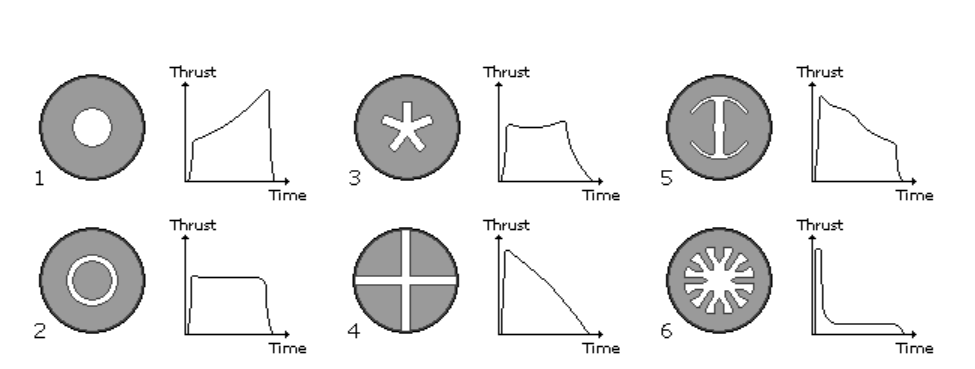
\includegraphics[width=0.7\linewidth]{figures/potentialShapes.png}
        \caption{Different thrust profiles may result in very different potential internal configurations of the rocket.
        Image courtesy of Robert A. Braeunig.}
        \label{fig:potentialShapes}
    \end{center}
\end{figure}


    \section{Geometry in polar coordinates}

Frankly, I underestimated the difficult algebra required to approximate
arc lengths and areas in polar coordinates. So I will detail it here
before I describe the constraints in my problem. Assuming that we
know the radius of our shape $r(\theta)$ for $\theta=[-\pi, pi]$,
the circumference and area of the shape is described as follows.

\begin{align}
    L & = \int\limits_{\pi}^{\pi} \sqrt{r^2 + \Big(\frac{dr}{d\theta}\Big)^2} d\theta \\
    A & = \int\limits_{\pi}^{\pi} r^2 d\theta
\end{align}

This poses some problems, since the integral of the square root of a polynomial
is not a polynomial that is amenable to \gls{sos} representation, since the
constraints need to be linear over the coefficients of the polynomial.


    \section{Sample output of first stage model}

This was only the first of the many hurdles I faced. This is not completely a surprise,
due to the complex nature of internal combustion
models, but the first stage model was quite fragile. It is highly sensitive to
input parameters and initial guesses, and the existence of a rocket with a given
burn profile is not
guaranteed even with significant relaxations of the conservation laws. However, I was
able to extract aggregate geometric information for a constant burn rocket, which I present
here and use in the rest of the project. The rocket in question burns at a constant thrust
of $150\rm{kN}$ for 4 seconds. The area and circumference evolution of the cross section of the rocket
are shown in Figure~\ref{fig:profiles}.

\begin{figure}
    \begin{subfigure}{0.48\textwidth}
        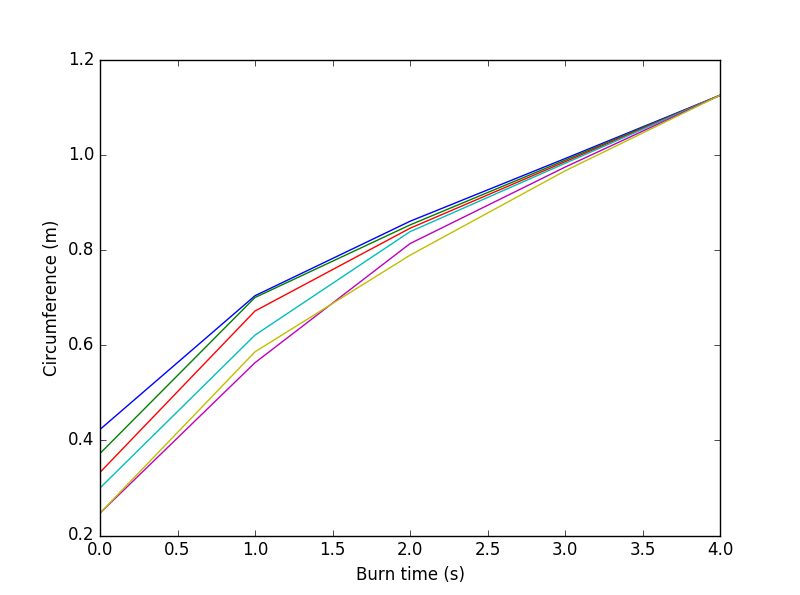
\includegraphics[width = 0.9\linewidth]{figures/cprofile.png}
        \caption{Cross-sectional circumference evolution}
        \label{fig:csec}
    \end{subfigure}
    \begin{subfigure}{0.48\textwidth}
        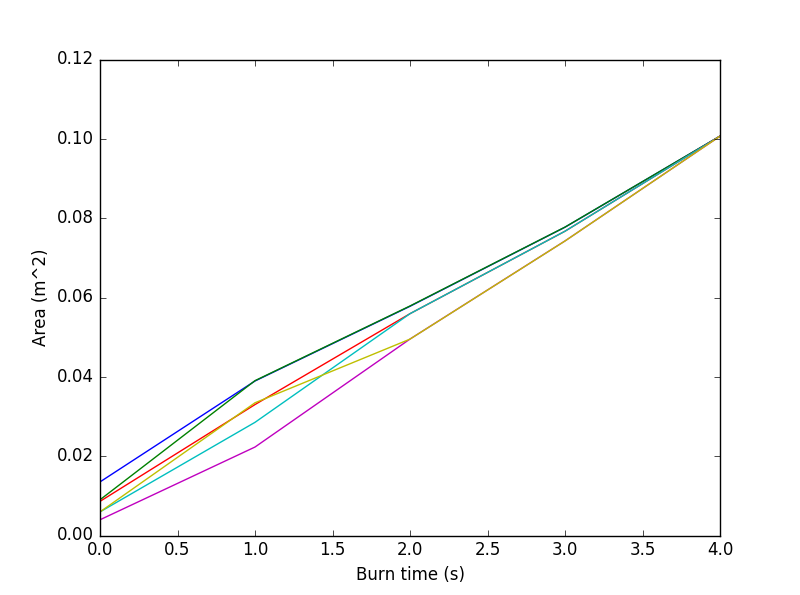
\includegraphics[width = 0.9\linewidth]{figures/aprofile.png}
        \caption{Cross-sectional area evolution}
        \label{fig:asec}
    \end{subfigure}
    \caption{Evolution of the cross-section of the rocket at 6 axial locations.}
    \label{fig:profiles}
\end{figure}

For the rest of the report, we will be focusing on mapping the cross-sectional
area and circumference evolution of the blue curve onto polynomials.


       \section{Constraint definition}
   \label{sec:generalconstraints}

    This section elaborates on the general form of the constraints of the problem.
    The constraints are imposed at $n_x+1$ cross-sections to determine the polynomials describing
    the square of the radius at different cross-sectional slices of the rocket.
    The surface geometry in between the sections will be described through interpolation.

    \begin{itemize}
        \item \textbf{The integral difference between the cross-sectional areas of the shape must be equal
        to the fuel burnt in a given time step, as determined by the first-stage problem.} In other words
        for the $i$th slice of the rocket:
        \begin{equation}
            \int\limits_{-\pi}^{\pi} r_{i,t}^2 d\theta = A_{i,t}
        \end{equation}
        We can easily represent this constraint by taking the integral of the polynomial $r_{i,t}^2(\theta)$
        which makes this a linear constraint on the coefficients of the polynomial.
        \item \textbf{The arc length of the polynomial must be equal to the arc length $l_b$ as determined
        by the first-stage problem.} The arc length of an arbitrary polynomial curve has no closed-form solution, so we
        have to use the integral form below:
        \begin{equation}
            C_{i,t} = \int\limits_{-\pi}^{\pi} \sqrt{r_{i,t}^2 + \Big(\frac{dr_{i,t}}{d\theta}\Big)^2} d\theta
        \end{equation}
        This integral form unfortunately has no \gls{sos} representation. This means
        that I will implement an outer loop problem to make sure that the polynomials
        have the appropriate arc lengths.
        \item \textbf{The shapes must never intersect.}
        Since the flame front must strictly regress as a result of burning,
        the polynomials describing the shapes must not intersect.
        This is a sum-of-squares constraint on the difference of the univariate polynomials, where
        $r^2_{i,t}(\theta) - r^2_{i,t-1}(\theta) \rm{~is~SOS~over~} \theta \in [-\pi, \pi]$.
        \item\textbf{The shapes must not intersect the unit circle.}
        Since fuel can only be contained inside the casing of the rocket,
        we set an upper bound on the polynomials. This can be achieved by making sure
        the polynomials don't intersect with the unit circle. This means that
        $R^2 - r^2_{i,n_t}(\theta) \rm{~is~SOS~over~} \theta \in [-\pi, \pi]$, where
        $R$ is the outer radius of the \gls{srm}.
        \item \textbf{Regularity conditions on the shape of the polynomials.}
        The first regularity condition is that the polynomials `close' over $[-\pi, \pi]$, i.e.
        that $r^2_{i,t}(-\pi) = r^2_{i,t}(\pi)$.
        I tried imposing conditions on the first and second derivative of the polynomial over the boundary as well,
        but this ended up making the problem less well-posed (solver SeDuMi kept running
        into numerical problems, the polynomials were not remotely close to satisfying constraints).
    \end{itemize}


    
    \section{Results}

Even the most basic area-fitting formulation posed problems for SeDuMi,
which was not able to solve the \gls{sos} problems to a satisfactory optimum
A sample solution is shown in Figure~\ref{fig:sampleSol}, for \gls{sos}
polynomials of order 12.

\begin{figure}
    \begin{subfigure}{0.48\textwidth}
        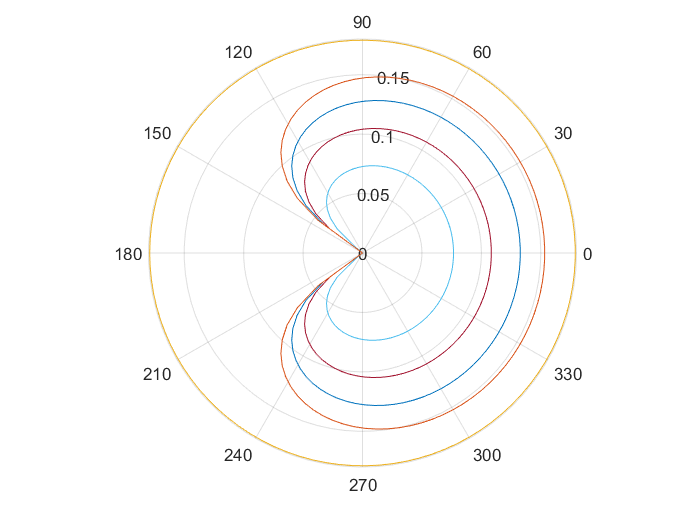
\includegraphics[width = 0.9\linewidth]{figures/sampleSol.png}
    \caption{The shape evolution of the polynomial shows a singulary at the boundaries $-\pi$ and $\pi$.}
        \label{fig:sampleSol}
    \end{subfigure}
    \begin{subfigure}{0.48\textwidth}
        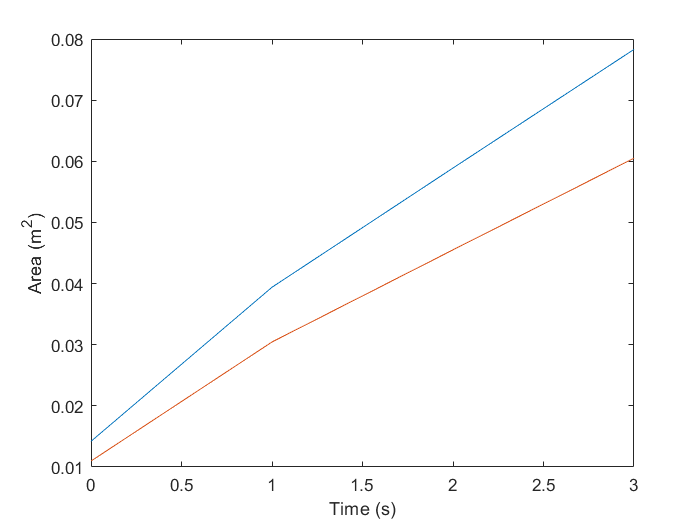
\includegraphics[width = 0.9\linewidth]{figures/sampleA.png}
        \caption{Cross-sectional area evolution of polynomials undershoots the constraints.}
        \label{fig:sampleA}
    \end{subfigure}
    \caption{The simple area-fitting formulation with only L0-continuous boundary condition
    on polynomial fails to return a satisfactory solution.}
    \label{fig:sampleSolandA}
\end{figure}

I believe this has a lot to do with the singularity at the boundary of the domain. This is occurring since the shape is
upper bounded by the outer radius of the rocket, but lower bounded by zero in the domain. I tried a
number of methods to stop a singularity from occurring at the boundary. These included:
\begin{itemize}
    \item Changing the polynomial degrees (odd and even, since my polynomials are
    \gls{sos} only over the interval).
    \item Adding additional regularity conditions (1st and 2nd derivative) at the boundary.
    \item Adding small perturbations at the boundary through inequality constraints.
    \item Making the negative Euclidian distance of the boundary value the objective.
\end{itemize}

None of these attempts worked, although I did notice that the error of the result went down with
increasing degree, so the solver was making some sort of progress.
This is especially odd since it is possible to determine by hand constant
functions $r^2(\theta \in [-\pi, \pi])$ (circles) which satisfy the area constraints,
and yet the \gls{sos} program could not find these.

Frankly, after many hours of tinkering, I am convinced that \gls{sos} programs are not the
right method to tackle this problem. My next step would have been to take
the polynomials, determine their arc lengths, and perturb them with periodic functions (sinusoids)
of appropriate magnitude depending on the distance between the polynomials to ensure that I satisfy
my arc length and area requirements within a specified tolerance.


    \section{Conclusion}

I think that shape optimization presents exciting frontiers for the use of \gls{sdp}s in engineering.
The state of the art in the engineering community in shape optimization still involves
taking an initial guess and perturbing it within an optimization loop, which is slow and
prone to getting stuck in local minima. Although I did not make a terrible amount of progress solving
the second stage of this
problem, it was fun to take real-world constraints
and try to formulate a tractable approximation of problem using what I have learned in 6.256.
It was a shame that I could not figure out a way to deal with the bilinearity in the
coefficients of $r(\theta)$ in the area constraint.

\end{document}
